\documentclass{beamer}
\usetheme{CambridgeUS}
\usecolortheme{rose}
\usepackage{braket}


\title{Computing P‐T Diagrams from First Principles}
\author{Max Tyler}
\institute{The University of Edinburgh}
\date{April 2018}
 
 
 
\begin{document}
{ 
\usebackgroundtemplate
{
	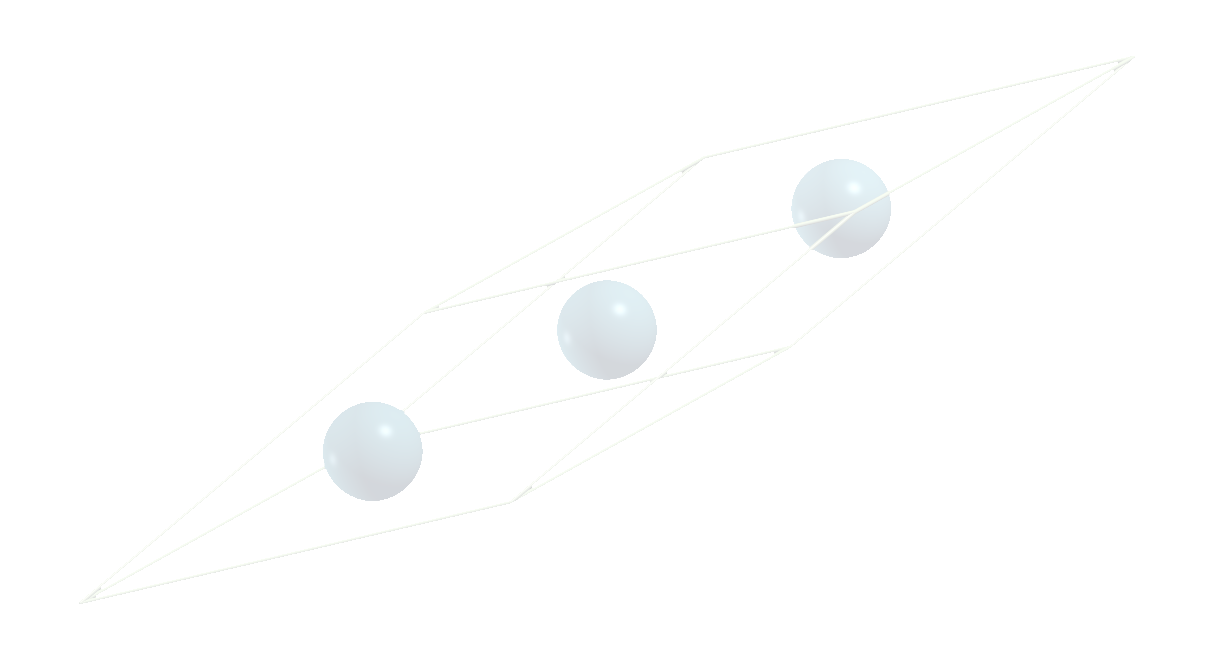
\includegraphics[width=\paperwidth,height=\paperheight]{na9rlarge.png}
}
\frame{\titlepage}
}
 
\begin{frame}
	\frametitle{PT Diagrams}
\end{frame}

\begin{frame}
	\frametitle{Density Functional Theory}
	Aim: Find the electron density, $n(\mathbf r)$ of some system.
	\begin{block}{Constrained Search for the Energy}<2->
		$$E_{v}[n] = \min_{\Psi \rightarrow n} \braket{\Psi|\hat T+\hat U + \hat V|\Psi} = F[n] + \int d^3\mathbf r n(\mathbf r) v_{ext}(\mathbf r)$$
	\end{block}
	\begin{block}{Kohn-Sham Formulation}<3->
		$$\left(-\frac{\hbar^2\nabla^2}{2m}+v_s(\mathbf r)\right)\phi_i(\mathbf r) = \epsilon_i \phi_i(\mathbf r),$$
		$$v_s(\mathbf r) = v_{ext}(\mathbf r) + v_H(\mathbf r) + v_{xc}(\mathbf r)$$
		$$n(\mathbf r) = \sum_i^N\phi^*_i(\mathbf r)\phi_i(\mathbf r)$$	
	\end{block}
\end{frame}

\begin{frame}
	\frametitle{Lithium Paper}
\end{frame}
 
\begin{frame}
	\frametitle{Silicon}
	\begin{figure}[ht]
	\begin{center}
	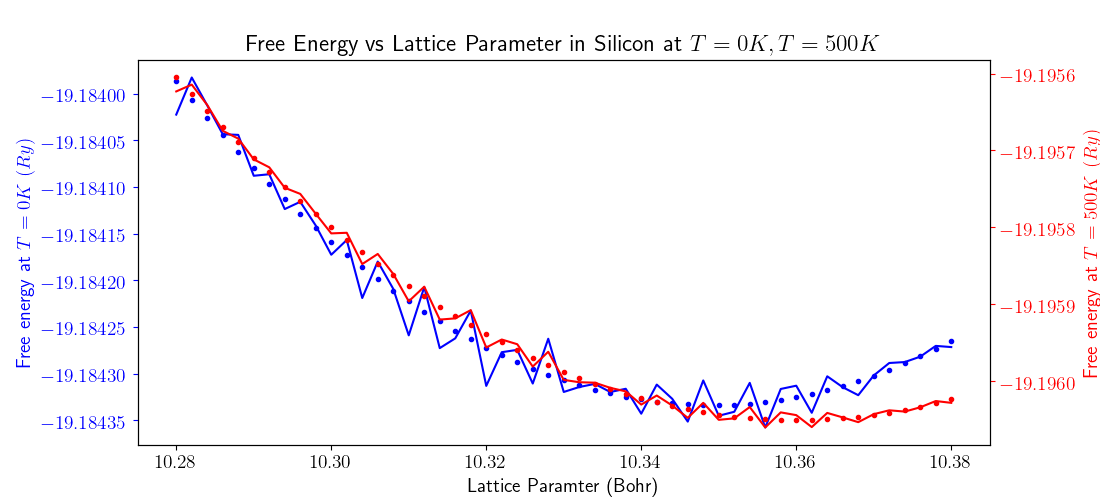
\includegraphics[height=2in]{silicon_0_500_comparison.png}
	\end{center}
	\end{figure}
\end{frame}

\begin{frame}
	\frametitle{Silicon}
	\begin{columns}
\column{0.5\textwidth}
	\begin{figure}[ht]
	\begin{center}
	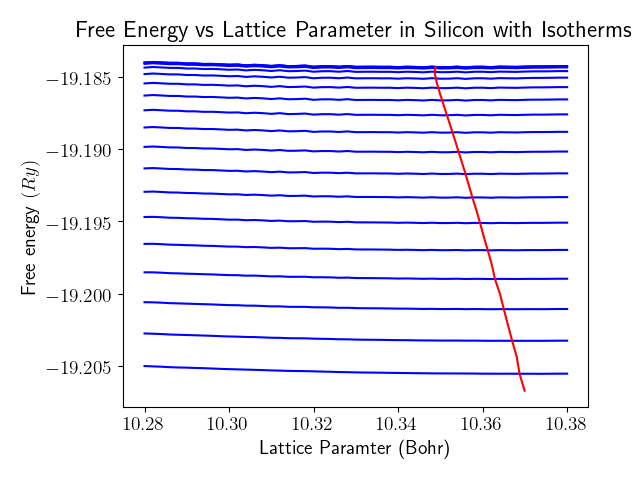
\includegraphics[height=1.8in]{silicon_isotherms.png}
	\end{center}
	\end{figure}
\column{0.5\textwidth}
	\begin{figure}[ht]
	\begin{center}
	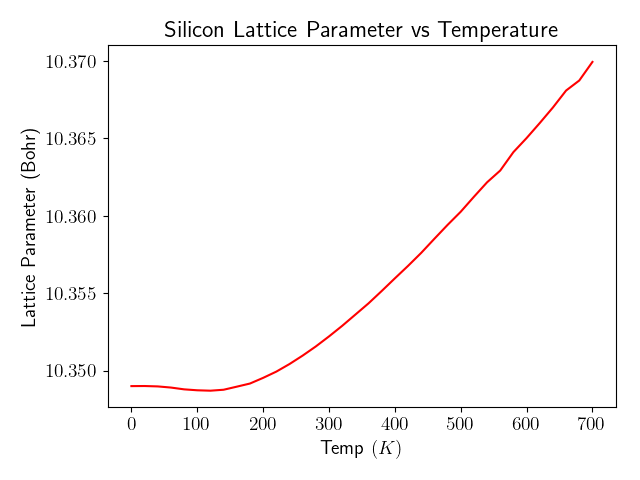
\includegraphics[height=1.8in]{silicon_min_volume.png}
	\end{center}
	\end{figure}
\end{columns}
\end{frame}

\begin{frame}
	\frametitle{Silicon \alpha}
	\begin{figure}[ht]
	\begin{center}
		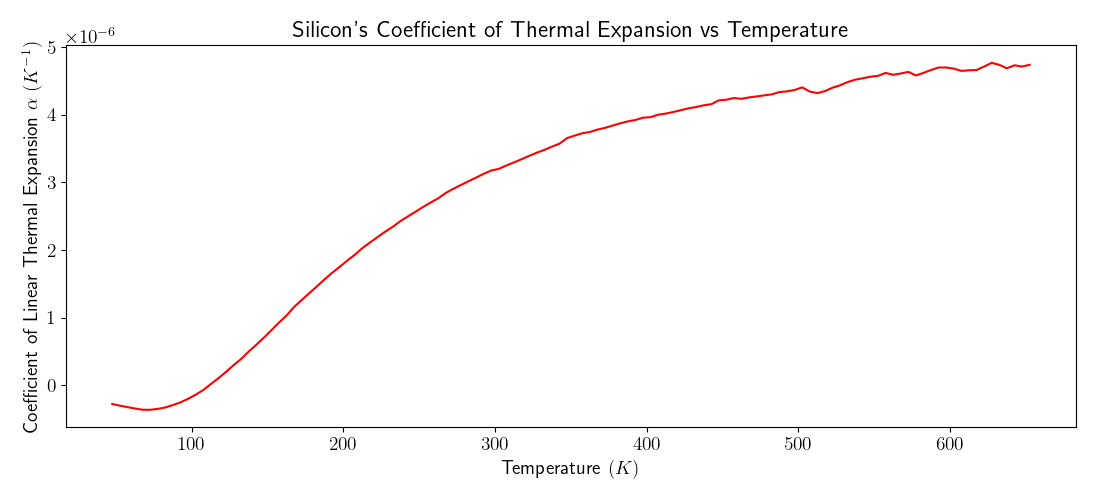
\includegraphics[height=1.8in]{silicon_thermal_expansion.png}
	\end{center}
	\end{figure}
\end{frame}

\begin{frame}
	\frametitle{Tin}
	\begin{figure}[ht]
	\begin{center}
	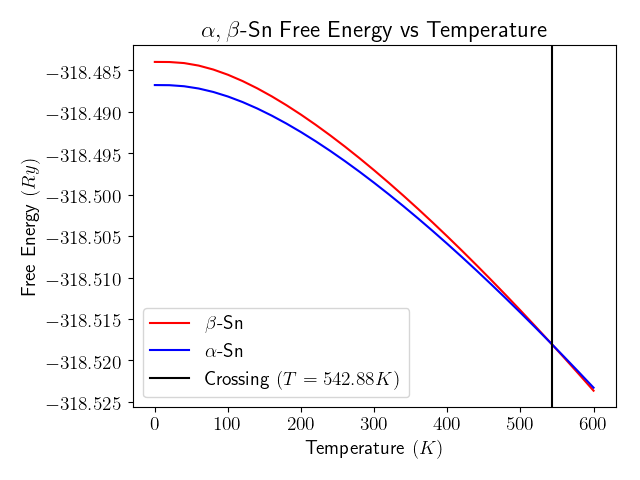
\includegraphics[height=2in]{tin_transition_temperature.png}
	\end{center}
	\end{figure}
\end{frame}

\begin{frame}
	\frametitle{Sodium Crystal Structure}
	\begin{columns}
\column{0.3\textwidth}
	\begin{figure}[ht]
	\begin{center}
		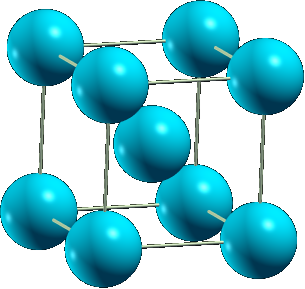
\includegraphics[height=1.3in]{nabcccrystal.png}
	\end{center}
	\end{figure}
	\begin{center}
		BCC
	\end{center}
\column{0.3\textwidth}
	\begin{figure}[ht]
	\begin{center}
		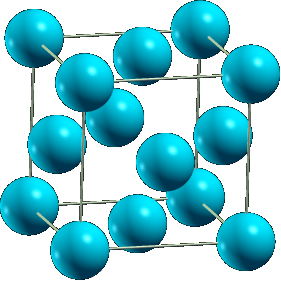
\includegraphics[height=1.3in]{nafcccrystal.png}
	\end{center}
	\end{figure}
	\begin{center}
		FCC
	\end{center}
\column{0.3\textwidth}
	\begin{figure}[ht]
	\begin{center}
		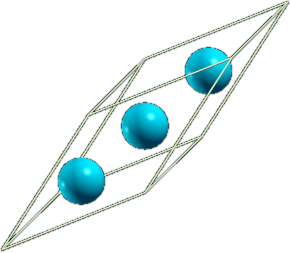
\includegraphics[height=1.23in]{na9rcrystal.png}
	\end{center}
	\end{figure}
	\begin{center}
		9R
	\end{center}
\end{columns}
\end{frame}
\begin{frame}
	\frametitle{Sodium PT Diagram}
	\begin{figure}[ht]
	\begin{center}
		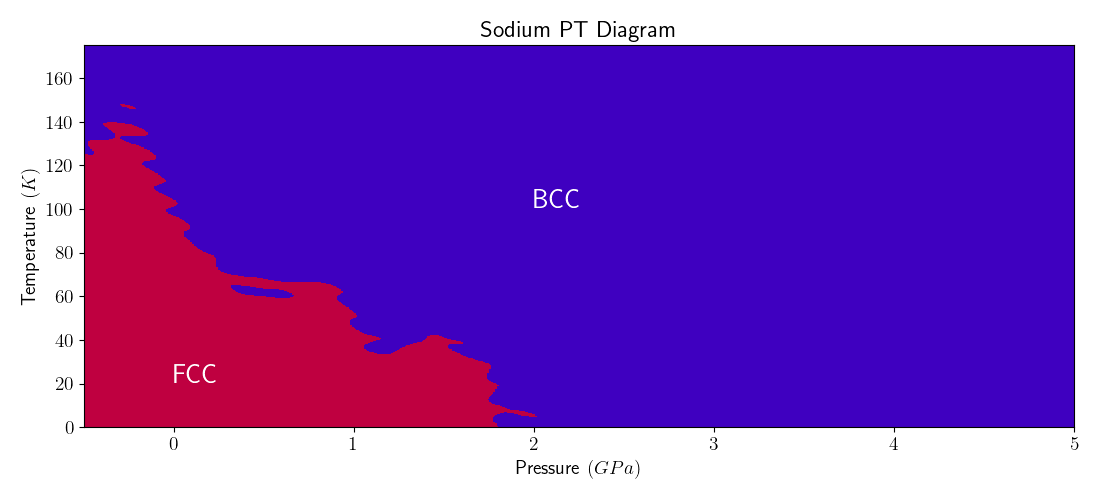
\includegraphics[height=2in]{sodium_pt_diagram.png}
	\end{center}
	\end{figure}
\end{frame}

\begin{frame}
	\frametitle{Not 9R Any More!}
\end{frame}

\begin{frame}
	\frametitle{Further Research}
	Look into other phases in this region (HCP, etc.)
\end{frame}

\end{document}

